% Slides for 2025-08-26
% To create a slide, use the following:
% \begin{frame}{TITLE}
%     BODY
% \end{frame}

% To create a slide with a bullet list, use the following:
% \begin{frame}{TITLE}
%     \begin{itemize}
%         \item ITEM 1
%         \item ITEM 2
%     \end{itemize}    
% \end{frame}

% To create a slide with numbered list, use the following:
% \begin{frame}{TITLE}
%     \begin{enumerate}
%         \item ITEM 1
%         \item ITEM 2
%     \end{enumerate}
% \end{frame}

% To create a slide with a graphic:
% 1. Add the graphic to this folder (named picture.png)
% 2. Use the following:
% \begin{frame}{TITLE}
%     \centering
%     \includegraphics[height=0.7\textheight,width=0.7\textwidth,keepaspectratio]{picture.png}
% \end{frame}

% To create a slide with two columns, use the following:
% \begin{frame}{TITLE}
%     \begin{columns}
%         \begin{column}{0.5\textwidth}
%             COLUMN 1 BODY
%         \end{column}
%         \begin{column}{0.5\textwidth}
%             COLUMN 2 BODY
%         \end{column}
%     \end{columns}
% \end{frame}

\begin{frame}{Strength in Numbers?}
  \begin{columns}
    \begin{column}{0.3\textwidth}
      \begin{itemize}
        \item LR and $R^2$
        \item ODR and MSE
        \item Mahalanoblis and $\chi^2$
      \end{itemize}
    \end{column}

    \begin{column}{0.7\textwidth}
      \raggedright    \includegraphics[height=0.7\textheight,keepaspectratio]{images/regression.png}
    \end{column}
  \end{columns}
\end{frame}

\begin{frame}{Depth Is All You Need}
    \centering
    \includegraphics[height=0.95\textheight,width=0.95\textwidth,keepaspectratio]{images/bullseye.png}
\end{frame}

\begin{frame}{Depth Anything Anything}
    \centering
    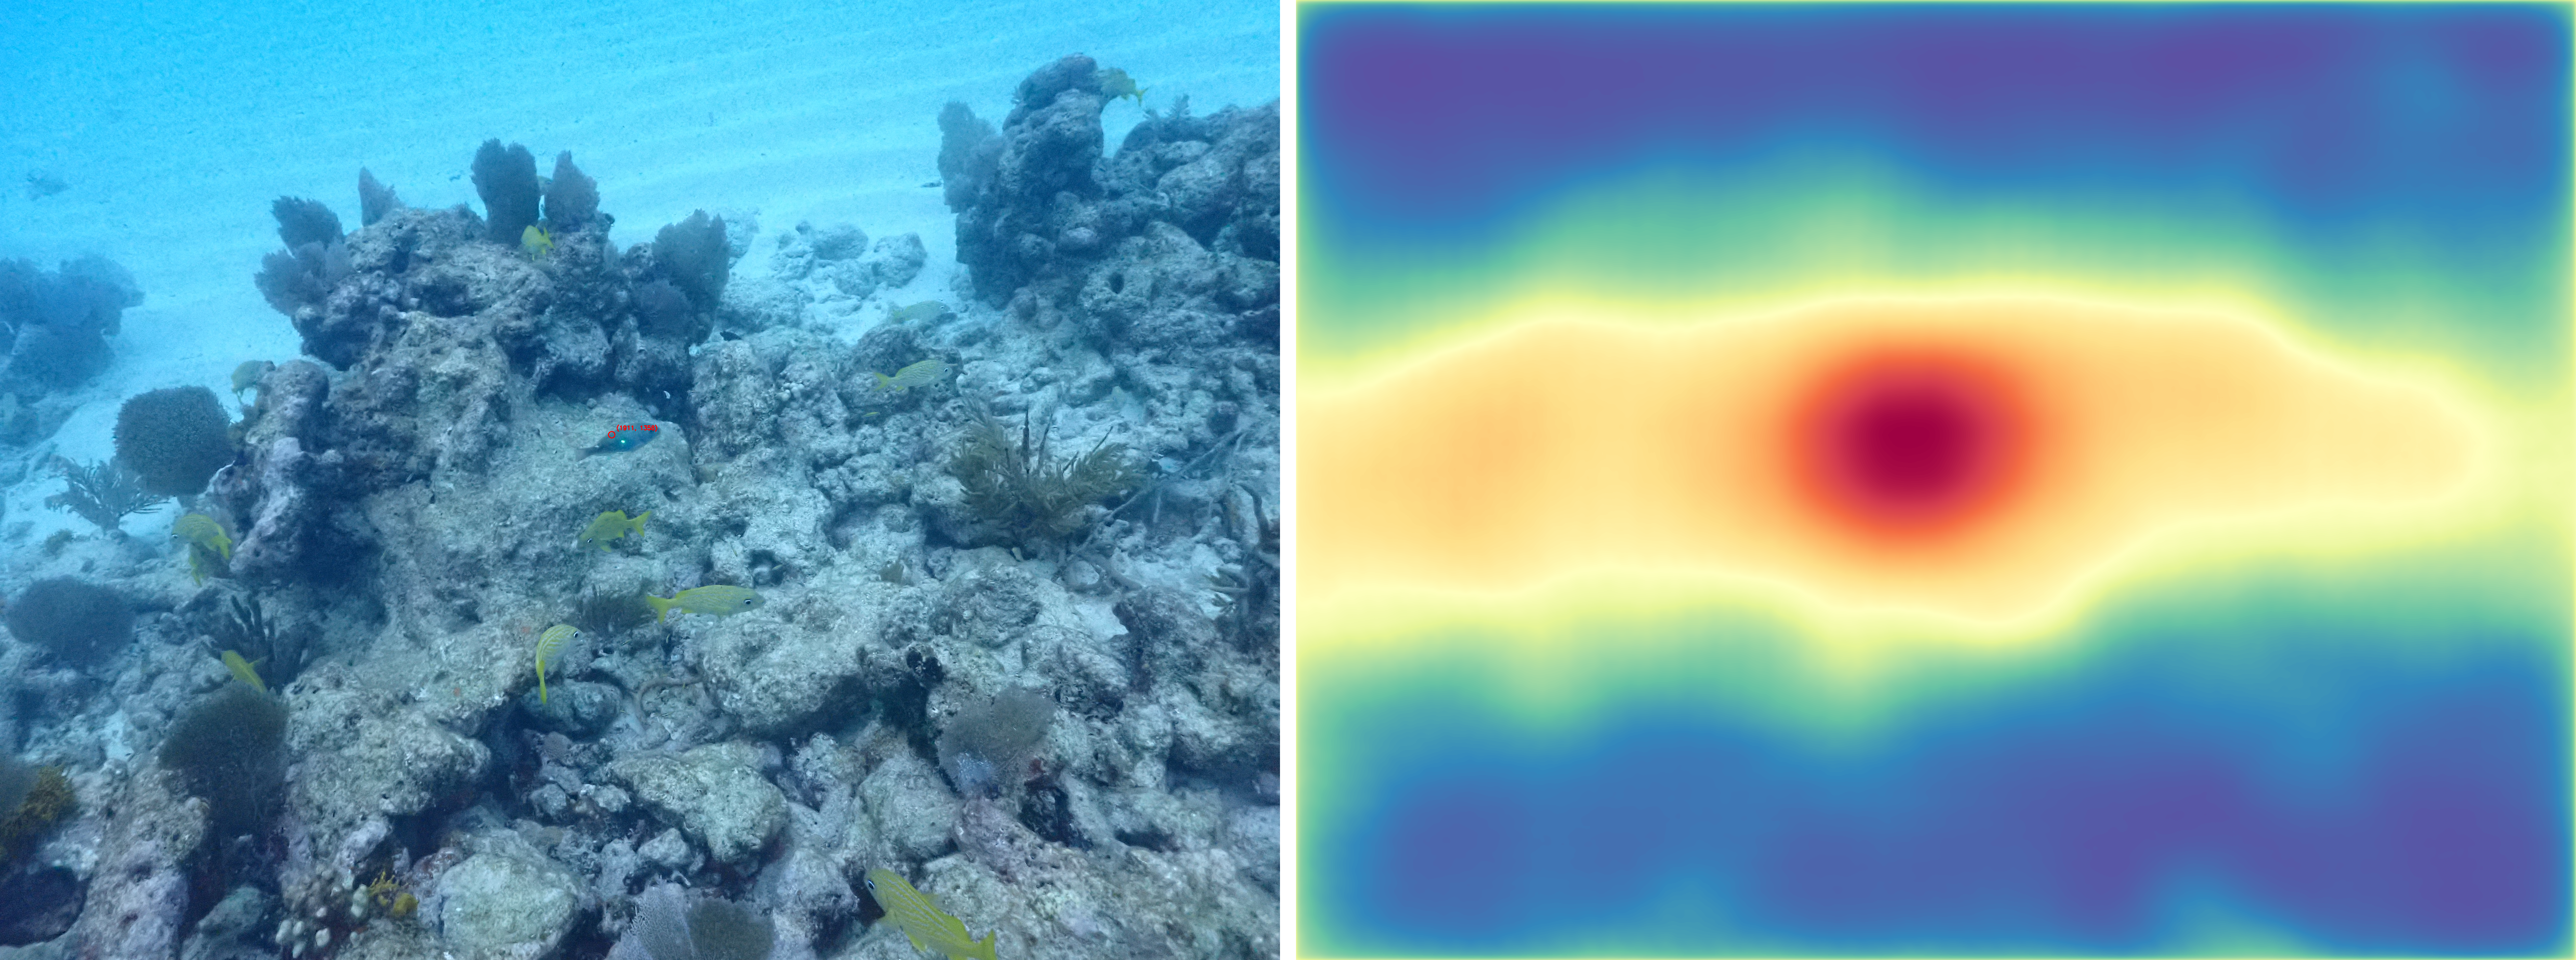
\includegraphics[height=0.95\textheight,width=0.95\textwidth,keepaspectratio]{images/detection.png}
\end{frame}

\begin{frame}{Perhaps You Can Tuna Fish}
    \centering
    \includegraphics[height=0.95\textheight,width=0.95\textwidth,keepaspectratio]{images/tuning.png}
\end{frame}

\begin{frame}{LiDAR SLAM}
    \begin{itemize}
        \item LiDAR SLAM combines multiple angles for better accuracy
    \end{itemize}

    \centering
    \includegraphics[height=0.7\textheight,keepaspectratio]{images/LiDAR SLAM.png}
\end{frame}
